\documentclass[../main]{subfiles}

\questiontrue
\solutiontrue

\begin{document}
    \ifquestion
    
    \section{Unfocused Photometry}
	
	Eugene, a Paraguayan telescope salesman, once bought a certain refracting telescope at a low price. Upon arriving home, he noticed that the telescope lens was terrible: the chromatic aberration was very large!
	
	He noticed this because he was observing different stars and saw that the lens focus was extremely variable. He collected the data in the following table:
	
	\begin{table}[htpb]
	    \centering
        \caption{Data of the temperature and focal distance of the rays from each star}
	    \begin{tabular}{c c c} 
			\toprule
			Star & Temperature (K) & Focus (cm) \\ 
			\midrule
			Spica & 25 000 & 3.11\\

			Betelgeuse & 3 600 & 149.93\\

			Aldebaran & 4 055 & 118.17\\

			Sirius & 9 845 & 20.05\\
			\bottomrule
		\end{tabular}
	    
	    \label{tab:starinfo}
	\end{table}

	
	Even frustrated with the purchase, he had an idea: to try to find information about a star from the undesired phenomenon. For this, he found a highly sensitive photoreceptor plate and placed it on the lens focal axis, observing the flux curve in relation to the distance (given in centimeters) to the center of the lens. The obtained curve was as follows:
	
	\begin{figure}[htpb]
	    \centering
	    \includegraphics[scale = 0.6]{images/mariobros.PNG}
	    \caption{Radiation intensity received by the photoreceptors as a function of the distance to the lens}
	    \label{fig:spectrum}
	\end{figure}


	
	Consider a known approximation for the refractive index of an object as a function of the wavelength of incident light:
	
	$$n(\lambda) = n_0+\frac{k}{\lambda^2}$$
	
	\ut{a} Determine the temperature of the star in question.
	
	
	
	To adjust the telescope, Eugene acquired two other lenses: A and B. Lens A has properties similar to the previous one, such that $$n_A(\lambda)=n_A+\frac{k_A}{\lambda^2}$$
	and lens B has a fixed focal distance $f_B$ (without chromatic aberration). In the following items, express your answers in terms of the presented parameters.
	
	\ut{b} Consider that the two curvature radii of a lens are equal ($R_1=R_2=R$). Find the relation between the curvature radii of the initial lens and lens A so that the optical system is stigmatic, i.e., has a well-defined focus.
	
	\ut{c} What is the maximum condition for $f_B$ so that the system functions as an objective lens?
	
	Tips:
	
	Can we approximate the value of $n_0$ from graphical analysis?
	
	Lens manufacturer equation:
	
	$$\frac{1}{f}=\left(\frac{n_{lens}}{n_{medium}}-1\right)\left(\frac{1}{R_1}+\frac{1}{R_2}\right)$$
	
	Combination of lenses placed very close together:
	
	$$\frac{1}{f_T}=\sum_i\frac{1}{f_i}$$
	
	\clearpage
    
    \fi
    
    \ifsolution
    
    \section{Unfocused Photometry}
	
	\ut{a} From the temperature of each star, we can find its respective wavelength of maximum emission (this is what we will use to relate to the focus) through Wien's law: $\lambda=\frac{0.0028976}{T}$. 
	From this, we find the relations for each star:
	
	\begin{table}[htpb]
	    \centering
     \caption{Data of wavelength adjusted from temperature and focal distance of the rays from each star}
	    \begin{tabular}{c c c} 
			\toprule
			Star & Wavelength ($\unit{\nano \meter}$) & Focus (cm) \\ 
			\midrule
			Spica & 115.90 & 3.11\\

			Betelgeuse & 804.89 & 149.93\\

			Aldebaran & 714.57 & 118.17\\

			Sirius & 294.32 & 20.05\\
			\bottomrule
		\end{tabular}
	    
	    \label{tab:starinfo2}
	\end{table}
	
	Assuming the refractive index of air is equal to 1 (a very good approximation), we want to find the refractive index of the lens for some cases. For this, we calculate the ratio of focal distances between any focus and a reference focus. Notice that the ratio between the reference focus and that of any star $i$ is of the form:
	
	$$\frac{f_r}{f_i}=\frac{n_0-1+\frac{k}{\lambda_i^2}}{n_0-1+\frac{k}{\lambda_r^2}}$$
	
	Let us define $\dfrac{f_r}{f_i}=y_i$, $\dfrac{1}{\lambda_i^2}=x_i$, $\dfrac{k}{n_0-1+\dfrac{k}{\lambda_r^2}}=a$ and $\dfrac{n_0-1}{n_0-1+\dfrac{k}{\lambda_r^2}}=b$
	
	From this we get:
	
	$$y_i=b+ax_i$$
	
	Performing a linear regression with all possible combinations\footnote{This is not really necessary at the moment, it is enough to find a single law, but it is interesting to see how all the lines behave.} we obtain the graphs in Figure \ref{fig:graph}.
	
	\begin{figure}[htpb]
	    \centering
	    \pgfplotsset{width = 12cm}
	    \begin{tikzpicture}
	    \begin{axis}[axis lines = left,
	       ylabel = {\Large$\dfrac{f_r}{f}$},
	       xlabel = {\Large$\lambda^{-2}$},
	       xmin = 0,
	       xmax = 8e-5,
	       ymin = 0, 
	       ymax = 50,
	       ytick distance = 10,
	       legend style = {font = \Large,
	                       at = {(0.1,0.9)},
	                       anchor = north west},
	   ]
	    
	    \addplot[color=red, domain = 0:8e-5]{1.34331e4*x-1.91033e-5};
	    
	    \addplot[color=black, domain = 0:8e-5]{64.75980e4*x-92.09508e-5};
	    
	    \addplot[color=teal, domain = 0:8e-5]{51.04159e4*x-72.58637e-5};
	    
	    \addplot[color=blue, domain = 0:8e-5]{8.660267e4*x-12.315789e-5};
	    
	    \legend{$Spica$, $Betelgeuse$, $Aldebaran$, $Sirius$}
	    
	    \addplot[color=red, only marks]coordinates{
	        (1/115.90^2, 1)
	        (1/(804.89^2), 3.11/149.93) %B
	        (1/(714.57^2), 3.11/118.93) %A
	        (1/(294.32^2), 3.11/20.05) %SI
	    };
	    %SPICA
	    
	    \addplot[color=black, only marks]coordinates{
	        (1/115.90^2, 149.93/3.11) %SP
	        (1/804.89^2, 1)
	        (1/714.57^2, 149.93/118.17) 
	        (1/294.32^2, 149.93/20.05)
	    };
	    %BETELGEUSE
	    
	    \addplot[color=teal, only marks]coordinates{
	        (1/115.90^2, 118.17/3.11)
	        (1/804.89^2, 118.17/149.93)
	        (1/714.57^2, 1)
	        (1/294.32^2, 118.17/20.05)
	    };
	    %ALDEBARAN
	    
	    \addplot[color=blue, only marks]coordinates{
	        (1/115.90^2, 20.05/3.11)
	        (1/804.89^2, 20.05/149.93)
	        (1/714.57^2, 20.05/118.17)
	        (1/294.32^2, 1)
	    };
	    %SIRIUS
	    
	    
	    \end{axis}
	    \end{tikzpicture}
	    \caption{Regression lines found for each pair of stars}
	    \label{fig:graph}
	\end{figure}
	

	From this we find the following lines for each reference star, in SI units:
	
	\begin{itemize}
		\item \textbf{Spica:} $y=1.34331\cdot10^{-14}x-1.91033\cdot10^{-5}$
		\item \textbf{Betelgeuse:} $y=64.75980\cdot10^{-14}x-92.09508\cdot10^{-5}$
		\item \textbf{Aldebaran:} $y=51.04159\cdot10^{-14}x-72.58637\cdot10^{-5}$
		\item \textbf{Sirius:} $y=8.660267\cdot10^{-14}x-12.315789\cdot10^{-5}$
	\end{itemize}
	
	Now we need to find the distance where the rays of highest intensity were focused. From the figure we can estimate this distance to be approximately $f=37.60$ cm (even though the graph is not perfectly linear, the local variation is small, so we can reasonably approximate it as linear locally). From this, we apply this value to the functions above and find the value of $x\  (\lambda^{-2}=x)$:
	
	
	
	\begin{itemize}
		\item \textbf{Spica:} $\lambda = 402.950 nm$
		\item \textbf{Betelgeuse:} $\lambda = 402.951 nm$
		\item \textbf{Aldebaran:} $\lambda = 402.950 nm$
		\item \textbf{Sirius:} $\lambda = 402.950 nm$
	\end{itemize}
	
	As the Chinese sage would say: "it's as if it was meant to work." Finally, we can calculate the average temperature of the star from the mean wavelength of maximum emission ($\lambda = 402.95 nm$):
	
	$$T=7190 K$$
	
	\ut{b} We notice that from the equations found previously, the linear coefficient of the found lines is very small, so we can approximate it to zero, so that $n_0 \approx 1$\footnote{Even though the slope is also very small, remember that the value of $x$ will be extremely large in most cases, so the product approximates a number with magnitude much larger than the linear coefficient, which can alter it}.
	
	From the lens combination relation we have:
	
	$$\frac{1}{f_t}=\frac{1}{f_A}+\frac{1}{f_B}+\frac{1}{f_0}$$
	
	$$\frac{1}{f_t}=\left(n_A-1+\frac{k_A}{\lambda^2}\right)\left(\frac{1}{R_1}+\frac{1}{R_2}\right)+\frac{1}{f_B}+\frac{k}{\lambda^2}\frac{2}{R}$$
	
	$$\frac{1}{f_t}=(n_A-1)\left(\frac{1}{R_1}+\frac{1}{R_2}\right)+\frac{1}{f_B}+\frac{k_A}{\lambda^2}\left(\frac{1}{R_1}+\frac{1}{R_2}\right)+\frac{2k}{\lambda^2 R}$$
	
	To make $f_t$ independent of $\lambda$, we want:
	
	$$\frac{k_A}{\lambda^2}\left(\frac{1}{R_1}+\frac{1}{R_2}\right)+\frac{2k}{\lambda^2 R}=0$$
	
	From which we find:
	
	$$\frac{1}{R_1}+\frac{1}{R_2}=-\frac{2k}{Rk_A}$$
	
	\ut{c} The condition that needs to be satisfied for the lens to act as a converging lens is that $f_t>0$:
	
	$$\frac{1}{f_t}=(n_A-1)\left(-\frac{2k}{Rk_A}\right)+\frac{1}{f_B}>0$$
	
	Finally:
	
	$$f_B<\frac{Rk_A}{2k(n_A-1)}$$
	
	\clearpage
    
    
    \fi
\end{document}
